% !TeX root = ../translation.tex

\section{试验结果}

在本节中,我们将报告我们的实验结果

\subsection{训练过程}

AE-OT模型的训练主要包括两个步骤:训练AE和寻找OT图。OT步骤是使用该算法的GPU实现来完成的,如第4节所述。在AE步骤中,在训练过程中,我们采用Adam算法[49]对中性网络的参数进行优化,学习速率为$0.003,\beta_1=0.5,\beta_2=0.999$。当$L^2$损失停止下降时,这意味着网络已经找到了一个良好的编码图,我们冻结编码器部分,并继续训练网络进行解码图。编码器冻结前后的训练损失见表(\ref{table:1})。接下来,为了从给定的分布(这里使用均匀分布)到潜在特征的分布中找到OT映射,我们从均匀分布中随机抽取$100N$个随机点来计算能量的梯度。这里,$N$是数据集的潜在特征的数量。此外,在实验中,$\theta_{ij}$被设置为对不同的数据集的不同。具体来说,对于MNIST和Fashion-MNIST数据集,$\theta_{ij}$被设置为$0.75$,而对于CIFAR-10和CelebA数据集,它分别被设置为$0.68$和$0.75$。
\begin{table}[!htbp]
	\caption{编码器冻结前后AEs的$L^2$损失}
	\label{table:1}
	\centering
	\begin{tabular}{@{}ccccc@{}}
		\toprule
		\multirow{2}{*}{Situation} & \multicolumn{4}{c}{Dataset}                \\ \cmidrule(l){2-5} 
		& MNIST  & Fashion-MNIST & CIFAR-10 & CelebA \\ \cmidrule(r){1-5}
		Before                     & 0.0013 & 0.0026        & 0.0023   & 0.0077 \\
		After                      & 0.0005 & 0.0011        & 0.0018   & 0.0074 \\ \bottomrule
	\end{tabular}
\end{table}

我们的AE-OT模型是在一个Linux平台上使用PyTorch实现的。所有实验均在GTX1080Ti上进行。

\subsection{传输映射的不连续性试验}

在这个实验中,我们想要检验我们的假设:在大多数实际应用中,目标测度的支持是非凸的,奇异集是非空的,概率分布映射沿奇异集是不连续的。

如图\ref{fig:12}所示,我们使用AE计算从CelebA数据集$(\sum,\nu)$到潜在空间Z的编码/解码映射;编码映射$f_{\theta}: \sum \to Z$在潜在空间上将$\nu$向前推到$(f_{\theta})_{\#}\mu$。在潜在空间中,我们基于第4节,$T: Z\to Z$中描述的算法计算OT映射,其中$T$将单位立方体$\zeta$中的均匀分布映射到$(f_{\theta})_{\#}\nu$。然后,我们从分布$\zeta$中随机抽取一个样本$z$,并使用解码映射$g_{\xi}:Z\to \sum$ 将$T(z)$映射到生成的人类面部图像$g_{\xi} \circ T(z)$。图\ref{fig:12}(a)展示了由该AE-OT框架生成的真实面部图像。

如果潜在空间中的推进测度$(f_{\theta})_{\#} \nu$的支持是非凸的,则会有一个奇异集$\sum _k$,其中$k>0$。我们想检测出$\sum _k$的存在。我们在潜在空间中随机抽取单位立方体中的线段,然后沿着这条线段进行密集插值,生成面部图像。如图\ref{fig:12}(b)所示,我们找到了一个线段$\gamma$,并在一个有一双棕色眼睛的男孩和一个有一对蓝眼睛的女孩之间生成了一个变形序列。在中间,我们生成了一张有一只蓝眼睛和一只棕色眼睛的脸,这绝对是不现实的,而且在$\sum$之外。这个结果意味着线段$\gamma$经过一个奇异集$\sum _k$,其中运输图$T$是不连续的。这也表明了我们的假设是正确的:编码的人脸图像测量在潜在空间上的支持是非凸的。

作为一个副产品,我们发现这个AE-OT框架提高了训练速度的5倍,并提高了收敛稳定性,因为OT步骤是一个凸优化。因此,它为改进现有的GAN提供了一种很有前途的方法。

\subsection{模式崩溃比较}

由于合成数据集由显式分布和已知模态组成,因此可以准确地测量模态坍塌。我们选择了两个在之前的工作中研究或提出的合成数据集:一个二维网格数据集。

为了选择模态崩溃的测量度量,我们采用了三个以前使用的度量[50,51]。模式的数量计算由生成模型产生的样本所捕获的模式的数量。在这个度量中,如果在该模式的三个标准差内没有产生样本,则被认为是丢失的。高质量样本的百分比衡量在最近模式的三个标准差内产生的样本的比例。第三个度量标准,在参考文献中使用。[51],是反向回-莱布勒(KL)散度。在这个度量中,每个生成的样本被分配到其最近的模式,并且我们计算分配在每个模式上的样本的直方图。然后,该直方图形成一个离散分布,然后计算其与真实数据形成的直方图的KL散度。直观地说,这衡量了生成的样本在真实分布的所有模式之间的平衡程度

在参考文献中。[51],作者用上述三个指标评估了GAN[26]、ALI[52]、MD[30]和PacGAN[51]。每个实验都在相同的生成器架构下进行训练,总共有大约400k的训练参数。这些网络在100k个样本上被训练了400个时代。对于AE-OT实验,由于源空间和目标空间都是二维的,因此不需要训练AE。我们直接计算了一个半离散的OT,它映射在单位平方上的均匀分布和经验的真实数据分布之间。理论上,OT恢复所有模式所需的最小真实样本量是每个模式一个样本。然而,这可能会导致在插值过程中产生低质量的样品。因此,对于OT计算,我们取512个真实样本,并基于此映射生成新的样本。我们注意到,在这种情况下,在OT计算中只有512个参数需要优化,并且由于凸正定黑森的存在,优化过程是稳定的。我们的结果在表(\ref{table:2})中所示,以前的方法的基准测试是从参考文献中复制出来的。[51]为了说明这一点,我们在图\ref{fig:13}中绘制了与GAN和PAcGAN一起绘制的合成数据集上的结果。
\begin{table}[!htbp]
	\caption{二维网格数据集的模式折叠比较}
	\label{table:2}
	\centering
	\begin{tabular}{@{}cccc@{}}
		\toprule
		& Modes       & Samples       & Reverse KL     \\ \midrule
		GAN     & 17.3\pm 0.8  & 94.8 \pm 0.7\% & 0.70 \pm 0.07   \\
		ALI     & 24.1 \pm 0.4 & 95.7 \pm 0.6\% & 0.14 \pm 0.03   \\
		MD      & 23.8 \pm 0.5 & 79.9 \pm 3.2\% & 0.17 \pm 0.003  \\
		PacGAN2 & 23.8 \pm 0.7 & 91.3 \pm 0.8\% & 0.13 \pm 0.04   \\
		PacGAN3 & 24.6 \pm 0.4 & 94.2 \pm 0.4\% & 0.06 \pm 0.02   \\
		PacGAN4 & 24.8 \pm 0.2 & 93.6 \pm 0.6\% & 0.04 \pm 0.01   \\
		AE-OT   & 25.0 \pm 0.0 & 99.8 \pm 0.2\% & 0.007 \pm 0.002 \\ \bottomrule
	\end{tabular}
\end{table}

\begin{figure}[h]
	\centering
	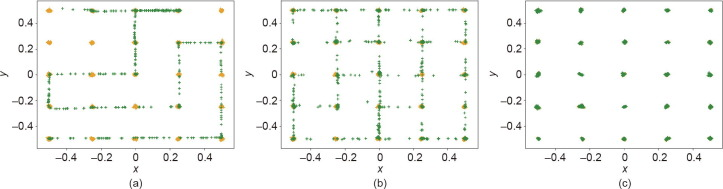
\includegraphics[width=0.6\linewidth]{13.jpg}
	\caption{2D格点数据集上的模式崩溃比较。(a)GAN;(b)PacGAN4;(c)AE-OT。橙色点代表真实样本,绿色点代表生成样本。}
	\label{fig:13}
\end{figure}

\subsection{与现有技术水平的比较}

我们设计了实验来比较我们提出的AE-OT模型与最先进的生成模型,包括由Lucic等人评估的对抗性模型。[33],以及Hoshen和Malik研究的非对抗性模型。[36].

为了进行公平的比较,我们使用了相同的测试数据集和网络体系结构。这些数据集包括MNIST[53]、MNIST-Dashion[54]、CIFAR-10[55]和CelebA[56],与在Refs中测试的数据类似。[31,36].该网络架构与Lucic等人在参考文献中使用的类似。[33].特别是,在我们的AE-OT模型中,解码器的网络结构与Ref中GANs的生成器相同。[33],编码器与解码器对称。

我们使用FID评分[31]和PRD曲线作为评价标准,将我们的模型与最先进的生成模型进行了比较。FID评分衡量生成结果的视觉保真度,并对图像损坏具有鲁棒性。然而,FID评分对模式的添加和删除[33]很敏感。因此,我们也使用了PRD曲线,它可以量化真实数据集[32]上的模式下降程度。

\subsubsection{与FID评分的比较}

FID得分的计算方法如下:\textcircled{1} 通过运行初始网络[30]提取生成的图像和真实图像在视觉上有意义的特征;\textcircled{2} 用高斯分布拟合真实和生成的特征分布;\textcircled{3} 使用以下公式计算两个高斯分布之间的距离:
\begin{equation}
	FID = \left \| u_r - u_g \right \|_2^2 + T_r \left [ \sum_r + \sum_g - 2\left ( \sum_r \sum_g \right )^{\frac{1}{2} }  \right ] 
	\label{function:34}
\end{equation}
其中,$\mu _r$和$\mu _g$分别表示真实分布和生成分布的平均值;$\sum _r$和$\sum _g$表示这些分布的方差

比较结果汇总见表(\ref{table:3})和表(\ref{table:4})。各种GANs的统计数据来自Lucic等人的[33],而非对抗性生成模型的统计数据来自Hoshen和Malik[36]。总的来说,我们提出的模型比其他最先进的生成模型获得了更好的FID分数。
\begin{table}[!htbp]
	\caption{与FID-I进行的定量比较}
	\label{table:3}
	\centering
	\begin{tabular}{@{}cclccl@{}}
		\toprule
		\multirow{2}{*}{Dataset} & \multicolumn{5}{c}{Adversarial}                 \\ \cmidrule(l){2-6} 
		& MM GAN & NS GAN & LS GAN & WGAN & BEGAN         \\ \cmidrule(r){1-6}
		MNIST                    & 9.8    & 6.8    & 7.8    & 6.7  & 13.1          \\
		Fashion-MNIST            & 29.6   & 26.5   & 30.7   & 21.5 & 22.9          \\
		CIF AR-10                & 72.7   & 58.5   & 87.1   & 55.2 & 71.4          \\
		CelebA                   & 65.6   & 55.0   & 53.8   & 41.3 & \textbf{38.9} \\ \bottomrule
	\end{tabular}
\end{table}

最佳结果以粗体显示。

\begin{table}[!htbp]
	\caption{与FID-II之间的定量比较}
	\label{table:4}
	\centering
	\begin{tabular}{@{}ccccccc@{}}
		\cmidrule(r){1-7}
		\multirow{2}{*}{Dataset} & \multicolumn{3}{c}{Non-adversarial} &  & \multicolumn{2}{c}{Reference} \\ \cmidrule(lr){2-4} \cmidrule(l){6-7} 
		& VAE        & GLO       & CLANN      &  & AE        & AE-OT             \\ \cmidrule(r){1-7}
		MNIST                    & 23.8       & 49.6      & 8.6        &  & 5.5       & \textbf{6.4}      \\
		Fashion-MNIST            & 58.7       & 57.7      & 13.0       &  & 4.7       & \textbf{10.2}     \\
		CIF AR-10                & 155.7      & 65.4      & 46.5       &  & 28.2      & \textbf{38.1}     \\
		CelebA                   & 85.7       & 52.4      & 46.3       &  & 67.5      & 68.4(\textbf{28.6})        \\ \cmidrule(r){1-7}
	\end{tabular}
\end{table}

最佳结果以粗体显示。

理论上,我们的AE-OT模型的FID分数应该与预先训练过的AEs模型的分数很接近;我们的实验也验证了这一点。

我们的AE的固定网络架构采用了Lucic等人的[33];它的容量不足以编码CIFAR-10或CelebaA,所以我们不得不对这些数据集进行降采样。我们从CIFAR-10中随机选择25k图像,从CelebA中选择10k图像来训练我们的模型。即便如此,我们的模型在CIFAR-10中获得了最好的FID分数。由于InfoGAN模型的有限容量,CelebA的AE性能的FID为67.5并不理想,进一步导致生成的数据集的FID为68.4。通过在AE体系结构中增加两个卷积层,CelebA的$L^2$损失小于$0.03$,FID得分优于其他所有的模型($28.6$,如表(\ref{table:4})的括号所示)。

\begin{figure}[h]
	\centering
	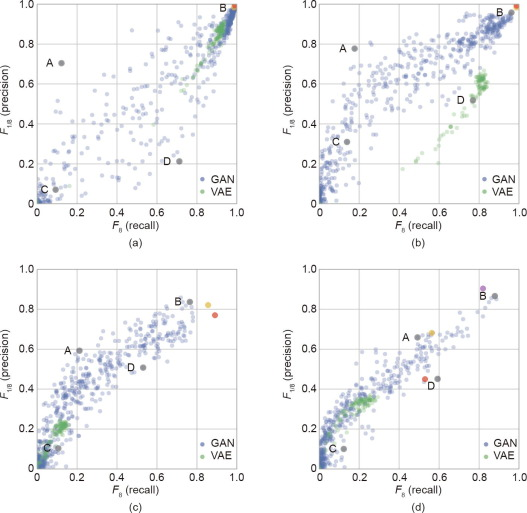
\includegraphics[width=0.6\linewidth]{14.jpg}
	\caption{在四个数据集上,以(F8, F1/8)的精确度-召回率进行比较。(a)MNIST;(b)FASHION;(c)CIFAR-10;(d)CelebA。黄褐色的点表示参考文献[36]中的结果。红色的点是利用本文所提出的方法生成的结果。(d)中紫色的点代表添加两个卷积层后,利用本文所提出的方法生成的结果。}
	\label{fig:14}
\end{figure}

\subsubsection{与PRD曲线的比较}

FID评分是衡量生成分布与真实数据分布差异的有效方法,但它主要关注精度,不能准确地捕获生成模型可以覆盖的真实数据的哪个部分。参考文献中提出的方法。[32]将分布之间的差异分解为两个组成部分:精度和召回率。

给定一个参考分布P和一个学习到的分布$Q$,精度直观地衡量从$Q$中获得的样本的质量,而召回率则衡量$Q$所覆盖的$P$的比例。

我们使用了Sajjadi等人在参考文献中提出的($F_8$,$F_{1 \setminus  8}$)的概念。[32]来量化精度和查全率的相对重要性。图\ref{fig:14}总结了比较结果。每个点代表一个具有一组超参数的特定模型。一个点越靠近右上角,模型的性能就越好。蓝色和绿色的点表示参考文献中评估的GANs和VAEs。[32],黄点代表Ref中的GLANN模型。[36],红点是我们的AE-OT模型.

很明显,我们提出的模型在MNIST和Dashion-MNIST上优于其他模型。对于CIFAR-10数据集,我们的模型的精度略低于GANs和GLANN,但查全率最高。对于CelebA数据集,由于AE的容量有限,我们的模型的性能并不令人印象深刻。然而,在AE中增加了两个卷积层后,我们的模型获得了最好的分数。

\subsubsection{视觉比较}

图\ref{fig:15}显示了我们提出的方法生成的图像与Lucic等人研究的GAN生成的图像之间的视觉比较。[33]和Hoshen和Malik研究的非对抗性模型。[36].第一列显示了原始图像,第二列显示了AE生成的结果,第三列显示最好的生成结果的差距在Lucicetal.[33],第四列显示所生成的结果霍申和马利克[36]的模型,和第五列显示我们的方法的结果。很明显,我们的方法可以生成高质量的图像,并覆盖了所有的模式。

\begin{figure}[h]
	\centering
	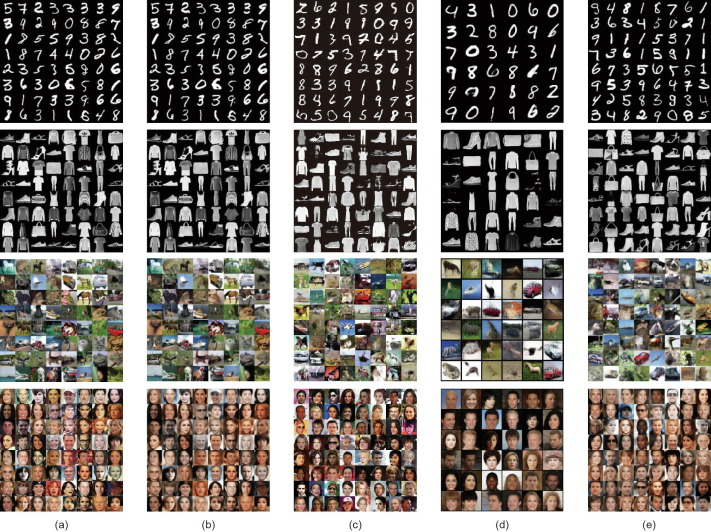
\includegraphics[width=0.6\linewidth]{15.jpg}
	\caption{生成图像质量在 4 个数据集上的可视化比较。第一列(a)是真实数据;第二列(b)是由AE生成的结果;第三列(c)显示的是由GAN[33]以最高的精确度-查全率$(F_8,F_{1 \setminus 8})$生成的结果,它对应着图\ref{fig:14}中的B点;第四列(d)是参考文献[36]中的结果;最后一列(e)是利用本文所提出的方法生成的结果。}
	\label{fig:15}
\end{figure}